\chapter{Ergebnisse und Auswertung}
\label{cha:Versuchsauswertung}


\section{Untersuchung des C-Faktors}
\label{sec:Untersuchungc-faktor}
In diesem Kapitel wird untersucht, wie der C-Faktor die Sprinklerauslösezeit bei variierendem Brandintensitätskoeffizient, Raumhöhe und RTI beeinflusst. Es soll ein Wärmeleitfaktor ermittelt werden, der die Sprinklerauslösezeiten am besten vorhersagt und in den nächsten Kapiteln verwendet werden kann. 
In den nachfolgenden Diagrammen wird der C-Faktor der Auslösezeit gegenübergestellt. Hierfür werden die Ergebnisse mit den Rechenergebnissen des SFPE Handbook 3rd Ed. und den Tabellenwerten der VDI 6019-1 verglichen. Zusätzlich werden die Ergebnisse mit der bestehenden Literatur abgeglichen. 

Die Tabellenwerte aus der VDI wurden allesamt mit einem C-Faktor von 0,7~(m/s)$^{0,5}$ errechnet. Da in den Berechnungen nach SFPE Handbuch kein C-Faktor einfließt, werden die Ergebnisse als durchgezogene Geraden in den Diagrammen dargestellt.  Alle Simulationen werden mit einem vertikalen Sprinklerabstand $r$ von 3,25 m und mit C-Faktoren von 0,0/0,5/1,0 und 1,5~(m/s)$^{0,5}$ durchgeführt. 



\subsection{Variierender Brandintensitätskoeffizient}

Die Simulationen mit variierendem Brandintensitätskoeffizient werden mit einer Raumhöhe von 3 m und einem RTI des Sprinklerkopfes gleich 50~(m$\cdot$s)$^{0,5}$ durchgeführt. In Abb.~\ref{fig:Ergebnisse_C-Faktor_Alphas} ist zu erkennen, dass der Einfluss des C-Faktors bei abfallendem Brand\-in\-ten\-si\-täts\-ko\-ef\-fi\-zien\-ten zunimmt. Aufgrund der damit einhergehenden langsameren Erwärmung des Auslöseelements besteht mehr Zeit, die Wärme an den Sprinklerkopf abzugeben und der Wärmeleitfaktor steigt in seiner Bedeutung.
Außerdem ist eine annähernd lineare Steigerung der Auslösezeit bei steigendem C-Faktor zu bemerken.
Die Sprinklerauslösezeiten der Simulationen bei einem $\alpha$ von 0,188 kW/s² und einem C-Faktor von 0,65~(m/s)$^{0,5}$ ähneln den Berechnungen nach SFPE Handbuch am meisten. Bei höheren Brand\-in\-ten\-si\-täts\-ko\-ef\-fi\-zien\-ten von 0,047~kW/s² und 0,188~kW/s² ist festzustellen, dass bei einem C-Faktor von 0~(m/s)$^{0,5}$ die höchste Übereinstimmung der Auslösezeit der Simulation mit den SFPE-Berechnungen vorliegt. Abschließend ist zu bemerken, dass die Tabellenwerte aus der VDI-Tabelle sehr viel höher liegen als die Ergebnisse aus den Simulationen oder den Berechnungen nach SFPE Handbuch.


\begin{figure}
    \centering
    \includegraphics[width=0.83\textwidth]{images/Ergebnisse_C-Faktor_Alphas.pdf}
    \caption{Sprinklerauslösezeiten bei verschiedenen C-Faktoren und Brand\-in\-ten\-si\-täts\-ko\-ef\-fi\-zien\-ten ($H=3$~m, RTI $=50$~(m/s)$^{0,5}$).}
    \label{fig:Ergebnisse_C-Faktor_Alphas}
\end{figure}



\subsection{Variierende Raumhöhe}

Die Simulationen mit variierender Raumhöhe werden mit einem Brandintensitätskoeffizienten von 0,047 kW/s² und einem RTI des Sprinklerkopfes gleich 50~(m$\cdot$s)$^{0,5}$ durchgeführt. In Abb. \ref{fig:Ergebnisse_C-Faktor_Raumhoehen} sind die Raumhöhe und der C-Faktor die variablen Parameter. Es sind annähernd lineare Verläufe der Auslösezeiten über die verschiedenen C-Faktoren zu beobachten. Generell dauert die Aktivierung des Sprinklerkopfes bei steigender Raumhöhe länger. Dies wird in Kap. \ref{sec:VergleichRaumhöhen} näher betrachtet. Die Steilheit der Verläufe nimmt mit der Höhe des Raumes zu, wobei der Anstieg des Auslösezeit der Raumhöhe $H=6$~m und $H=8$~m sich ähnelt. Der Einfluss des C-Faktors bei den höheren Räumen ist größer, da auch hier mehr Wärme über einen längeren Zeitraum im Vergleich zu der niedrigeren Raumhöhe abgegeben werden kann.
Ein C-Faktor von 0~(m/s)$^{0,5}$ scheint zu den höchsten Übereinstimmungen mit den Berechnungen zu führen.  Die VDI-Tabellenwerte liegen alle mindestens 20~s über den Simulationen bei gleichem C-Faktor. 


\begin{figure}
    \centering
    \includegraphics[width=0.83\textwidth]{images/Ergebnisse_C-Faktor_Raumhoehen.pdf}
    \caption{Sprinklerauslösezeiten bei verschiedenen C-Faktoren und Raumhöhen ($\alpha=0{,}047$~kW/s², RTI $=50$~(m/s)$^{0,5}$).}
    \label{fig:Ergebnisse_C-Faktor_Raumhoehen}
\end{figure}

\subsection{Variierender RTI}

Die Simulationen mit variierendem RTI werden mit einem Brandintensitätskoeffizienten von 0,047 kW/s² und einer Raumhöhe gleich 3~m durchgeführt. RTI von 27~(m$\cdot$s)$^{0,5}$, 50~(m$\cdot$s)$^{0,5}$ und 120~(m$\cdot$s)$^{0,5}$ werden in Abb. \ref{fig:Ergebnisse_C-Faktor_RTI} untersucht. Auch hier sind annähernd lineare Verläufe der Auslösezeiten zu beobachten. Es ist anzumerken, dass der C-Faktor an Bedeutung verliert mit ansteigendem RTI. Eine Ursache hierfür könnte die größere Wärmekapazität des Auslöseelements sein. Da das Glasfässchen bei höheren RTI im Durchmesser zunimmt, kann es mehr Wärme aufnehmen und die Wärmeleitung zum Sprinklerkopf fällt weniger ins Gewicht. Dies muss weiterführend untersucht werden.
Ein C-Faktor von 0~(m/s)$^{0,5}$ führt zu den höchsten Übereinstimmungen mit den SFPE-Berechnungen. 
\begin{figure}
    \centering
    \includegraphics[width=0.83\textwidth]{images/Ergebnisse_C-Faktor_RTI.pdf}
    \caption{Sprinklerauslösezeiten bei verschiedenen C-Faktoren und RTI ($\alpha=0{,}047$~kW/s², $H=3$~m).}
    \label{fig:Ergebnisse_C-Faktor_RTI}
\end{figure}

\subsection{Auswertung}

Da für die weiteren Simulationen nur ein konstanter C-Faktor betrachtet werden soll und in dieser Arbeit keine realen Brandversuche durchgeführt werden, muss ein Blick auf bereits bestehende Untersuchungen des C-Faktors geworfen werden. In der Masterthesis von Bittern \cite{Bittern2004} wurde unter anderem untersucht, mit welchem Trägheitsindex in FDS die größten Übereinstimmungen mit den realen Brandversuchen erreicht wurden. Abb. \ref{fig:BitternC-Faktor} zeigt die Häufigkeit der prozentuellen Abweichung der Ergebnisse auf. Bittern unterscheidet zwischen Residential und Standard Response Sprinklerköpfen. Die in dieser Arbeit verwendeten Residential Sprinklerköpfe weisen einen RTI von 36~(m$\cdot$s)$^{0,5}$ und die Standard Response Sprinklerköpfe einen RTI von 95~(m$\cdot$s)$^{0,5}$ auf. 
Auf der \emph{X-Achse} werden verschiedene C-Faktoren bei unterschiedlichen Sprinklerköpfen abgebildet. Die Balkenfarbe weißt darauf hin, ob Simulationen Abweichungen der Sprinklerauslösezeiten von 20~\%, 25~\% oder 30~\% zu den Real-Versuchen aufweisen.
Die \emph{Y-Achse} zeigt zusätzlich auf, wie viel Prozent der gesamten Simulationen Abweichungen mit den oben genannten Prozentzahlen zu den Real-Versuchen haben. Knapp über 90~\% der Simulationen weisen eine kleiner 20~\% Abweichung der Sprinklerauslösezeiten im Vergleich zu den entsprechenden Real-Versuchen mit Residential Sprinklerkopf bei einem C-Faktor von 0~(m/s)$^{0,5}$ auf.
Es ist dargelegt, dass ein C-Faktor von 0~(m/s)$^{0,5}$ die höchsten Übereinstimmungen mit den Realversuchen bei schnellauslösenden Sprinklerköpfen besitzt und 0,65~(m/s)$^{0,5}$ die höchsten Übereinstimmungen bei langsamer auslösenden Sprinklerköpfen. Weiterhin kann vermutet werden, dass auch bei den Standard Response Sprinklerköpfen ein niedrigerer C-Faktor zu höheren Übereinstimmungen führen würde. 

Da dieser Arbeit keine weiteren Untersuchungen des C-Faktors vorliegen und ein C-Faktor von 0~(m/s)$^{0,5}$ in FDS die Sprinklerauslösezeiten laut Bittern am besten vorhersagt, werden alle nachfolgenden Simulationen mit einem C-Faktor von 0~(m/s)$^{0,5}$ durchgeführt. Zusätzlich ist zu bemerken, dass die höchsten Übereinstimmungen zwischen der in diesem Kapitel durchgeführten Simulationen und Berechnungen, bei einem C-Faktor von 0~(m/s)$^{0,5}$ auftreten.


\begin{figure}
    \centering
    \includegraphics[width=\textwidth]{images/BitternC-Faktor.pdf}
    \caption{Gegenüberstellung der prozentuellen Abweichung von FDS-Simulationen und Realversuchen bei unterschiedlichen Sprinklerköpfen und C-Faktoren nach \cite{Bittern2004}.}
    \label{fig:BitternC-Faktor}
\end{figure}



\section{Vergleich Simulation und Berechnung}
\label{sec:VergleichSimulationundBerechnung}

In dieser Sektion werden die Sprinklerauslösezeiten der Simulationen bei unterschiedlichen Parametern mit den SFPE-Berechnungen und VDI-Tabellenwerten verglichen.

\subsection{Vergleich RTI}

Die nachfolgenden Simulationen werden mit einer Raumhöhe von 3~m und einem Brand\-in\-ten\-si\-täts\-ko\-ef\-fi\-zien\-ten von 0,047~kW/s² durchgeführt. 
Abb.~\ref{fig:RTIVergleich} zeigt den Verlauf der Sprinklerelementtemperaturen der Simulationen im Vergleich zu denen der SFPE-Berechnungen. Die Simulationsdatenpunkte werden als durchgezogene Linie und die Berechnungsdatenpunkte als punktierte Linie dargestellt. Die Sprinklerelementtemperaturen steigen alle exponentiell und versetzt zueinander an. Da Sprinklerauslöseelemente nur mit Nenn\-öff\-nungs\-tem\-pe\-ra\-tu\-ren von bis zu 260~°C von der VdS 2160 definiert werden, sind Betrachtungen über dieser Temperatur nicht notwendig. 

Je niedriger der RTI, desto steiler steigt die Elementtemperatur an. Es ist gut erkenntlich, dass bis ca. 170~s eine sehr hohe Übereinstimmung von Simulation zu Berechnung vorhanden ist. Ab diesem Zeitpunkt steigt die Temperatur aus den Simulationen schneller an als die aus den Berechnungen nach dem SFPE-Handbuch. Zu diesem Zeitpunkt scheint ein Schwall sehr heißen Rauchgases an dem Sprinklerkopf vorbeizuströmen. Dies lässt die Sprinklerelementtemperatur sprunghaft ansteigen. In Kap.~\ref{sec:VergleichRaumhöhen} wird dies genauer untersucht.

Tab.~\ref{tab:RTIErgebnisse} verdeutlicht die hohe Übereinstimmung der Simulationsergebnisse mit den Berechnungswerten. Erst ab Nennöffnungstemperaturen größer 141~°C kommt es zu Abweichungen größer 10~s. Zusätzlich kann auch die große Differenz zu den VDI-Tabellenwerten erkannt werden.


\begin{figure}
    \centering
    \includegraphics[width=\textwidth]{images/RTIVergleich.pdf}
    \caption{Verlauf der Sprinklerelementtemperatur bei verschiedenen RTI mit Vergleich zu Berechnungen nach SFPE Handbook ($\alpha=0{,}047$~kW/s², $H=3$~m).}
    \label{fig:RTIVergleich}
\end{figure}

\begin{table}\centering
\caption{Vergleich der Sprinklerauslösezeiten (in s) zwischen Simulationen, Berechnungen nach SFPE-Handbuch und VDI-Tabellenwerten für verschiedene Nennöffnungstemperaturen (Trd; in °C)  und RTI (in (m$\cdot$s)$^{0,5}$) ($\alpha=0{,}047$~kW/s², $H=3$~m).}
\label{tab:RTIErgebnisse}
\begin{tabu} to 0.85\textwidth{@{}X[c]X[c]X[c]X[c]X[c]X[c]X[c]X@{}} \toprule
   Trd &            & RTI 27 & RTI 50 & RTI 80 & RTI 120 & RTI 180 \\
    \midrule
    & Sim.       & 91     & 102    & 116    & 129     & 145     \\
 57 & SFPE       & 91     & 104    & 117    & 130     & 146     \\
    & VDI        & 125     & 140    & 150    & 165     & 175     \\
    \midrule
    & Sim.       & 102 & 116    & 129    & 144     & 159     \\
  68& SFPE       & 102    & 116    & 129    & 144     & 162     \\
    & VDI        & 145    & 155    & 170    & 185     & 196     \\
    \midrule
    & Sim.       & 114 & 126    & 141    & 154     & 171     \\
  79& SFPE       & 112    & 126    & 141    & 156     & 175     \\
    & VDI        & 165    & 175    & 185    & 200     & 215     \\
    \midrule
    & Sim.       & 126 & 140    & 153    & 168     & 180     \\
  93& SFPE       & 125    & 139    & 154    & 171     & 191     \\
    & VDI        & 185    & 195    & 205    & 220     & 235     \\
    \midrule
    & Sim.       & 161 & 189    & 182    & 200     & 217     \\
 141& SFPE       & 163    & 178    & 194    & 213     & 236     \\
    & VDI        & 245    & 255    & 270    & 285     & 300     \\
    \midrule
    & Sim.       & 178 & 191    & 210    & 223     & 245     \\
 182& SFPE       & 193    & 208    & 224    & 244     & 268     \\
    & VDI        & 295    & 305    & 315    & 335     & 350     \\
    \bottomrule
\end{tabu}
\end{table}

\FloatBarrier

\subsection{Vergleich Raumhöhen}
\label{sec:VergleichRaumhöhen}

Die nachfolgenden Simulationen werden mit einem RTI von 50~(m$\cdot$s)$^{0,5}$ und einem Brand\-in\-ten\-si\-täts\-ko\-ef\-fi\-zien\-ten von 0,047~kW/s² durchgeführt.
Abb. \ref{fig:RaumhoehenVergleich} zeigt den Verlauf der Sprinklerelementtemperaturen der Simulationen im Vergleich zu denen der SFPE-Berechnungen. Die Simulationsdatenpunkte werden als durchgezogene Linie und die Berechnungsdatenpunkte als punktierte Linie dargestellt. Es werden die Raumhöhen 3~m, 6~m und 8~m betrachtet. Aus den Kurven lässt sich ableiten, dass je größer die Raumhöhe ist, desto langsamer die Sprinklerelementtemperatur ansteigt. 
Während wie im vorherigen Abschnitt bereits besprochen eine Abweichung der Simulationsergebnisse von den Berechnungsergebnissen erst ab ca. 170~s zu beobachten ist, kommt es bei den anderen Raumhöhen schon früher zu geringen Abweichungen. Die Verläufe der Simulationen mit den beiden größeren Raumhöhen steigen ab ca. 150~s langsamer an als die Berechnungsverläufe im Gegensatz zum Verlauf der Raumhöhe mit 3~m. 

Obwohl die Simulationsergebnisse nur leicht versetzt zu den Berechnungsergebnissen sind, bedeutet der langsame Temperaturanstieg, dass schon geringe Abweichungen der beiden Datensätze zu großen Differenzen in den Auslösezeiten führen, wie in Tab. \ref{tab:RaumhoeheErgebnisse} zu erkennen ist. Auch wenn die Zeitunterschiede bei einer niedrigen Raumhöhe nur wenige Sekunden betragen, liegen die Abweichungen bei den Raumhöhen 6~m \bzw 8~m meist bei über 10~s.

\begin{figure}
    \centering
    \includegraphics[width=\textwidth]{images/RaumhoehenVergleich.pdf}
    \caption{Verlauf der Sprinklerelementtemperatur bei verschiedenen Raumhöhen mit Vergleich zu Berechnungen nach SFPE-Handbuch ($\alpha=0{,}047$~kW/s², RTI $=50$~m).}
    \label{fig:RaumhoehenVergleich}
\end{figure}

\begin{table}\centering
\caption{Vergleich der Sprinklerauslösezeiten (in s) zwischen Simulationen, Berechnungen nach SFPE-Handbuch und VDI-Tabellenwerten für verschiedene Nennöffnungstemperaturen (Trd; in °C)  und Raumhöhen ($\alpha=0{,}047$~kW/s², RTI $=50$~m).}
\label{tab:RaumhoeheErgebnisse}
\begin{tabu} to 0.7\textwidth{@{}X[c]X[c]X[c]X[c]X[c]X@{}} \toprule
Trd    &        &H = 3 m  & H = 6 m          & H = 8 m          \\
        \midrule
            & Sim.      & 102   & 143              & 170              \\
 57         & SFPE      & 104   & 135              & 157              \\
            & VDI       & 140   & 185              & 220              \\
          \midrule
            & Sim.      & 116   & 165              & 194              \\
 68         & SFPE      & 116   & 153              & 179              \\
            & VDI       & 155   & 210              & 250              \\
          \midrule
            & Sim.      & 126   & 183              & 212              \\
79          & SFPE      & 126   & 169              & 200              \\
            & VDI       & 175   & 240              & 285              \\
          \midrule
            & Sim.      & 140   & 210              & 259              \\
 93         & SFPE      & 139   & 189              & 226              \\
            & VDI       & 195   & 270              & 320              \\
          \midrule
            & Sim.      & 189   & 271              & \textgreater 300 \\
  141       & SFPE      & 178   & 252              & 306              \\
            & VDI       & 255   & 365              & 440              \\
          \midrule
            & Sim.      & 191   & \textgreater 300 & \textgreater 300         \\
 182        & SFPE      & 208   & 301              & 371            \\
            & VDI       & 305   & 440              & 535            \\
        \bottomrule
\end{tabu}
\end{table}

In den Abb. \ref{fig:GastempVergleich} und \ref{fig:GasgeschwVergleich} werden die Gastemperatur und Gasgeschwindigkeit am Sprinklerkopf näher betrachtet. Starke Unterschiede lassen sich bei der Temperatur beobachten. Im Schnitt fällt die Gastemperatur je höher der Abstand zwischen Brandherd und Decke ist. Da bei größerer Raumhhöhe mehr Umgebungsluft in den Plume induziert wird, kühlt der Plume stärker ab und der Volumenstrom an der Decke vergrößert sich. 
Eine stärkere Fluktuation der Rauchgastemperatur ist bei $H$~=~3~m ab ca. 170~s festzustellen, welche zum Teil über 300~K beträgt. Dies ist womöglich ein Grund für den starken Anstieg der Sprinklerelementtemperatur in Abb. \ref{fig:RaumhoehenVergleich}. Unregelmäßigkeiten wie diese sind eventuell auf eine Überschreitung des Plumes an einer Meshgrenze zurückzuführen. Auch eine numerische Instabilität der Simulation ab diesem Zeitpunkt ist nicht auszuschließen.

Die Rauchgastemperatur am Sprinklerkopf weist keine bedeutsamen Abweichungen bei unterschiedlicher Raumhöhe auf. Aus dem Diagramm kann jedoch abgeleitet werden, dass eine höhere Raumhöhe zu einer höheren Rauchgasgeschwindigkeit im Deckenbereich führt. 


\begin{figure}
    \centering
    \includegraphics[width=0.83\textwidth]{images/GastempVergleich.pdf}
    \caption{Verlauf der Rauchgastemperatur am Sprinklerkopf bei verschiedenen Raumhöhen.}
    \label{fig:GastempVergleich}
\end{figure}
\begin{figure}
    \centering
    \includegraphics[width=0.83\textwidth]{images/GasgeschwVergleich.pdf}
    \caption{Verlauf der Rauchgasgeschwindigkeit am Sprinklerkopf bei verschiedenen Raumhöhen.}
    \label{fig:GasgeschwVergleich}
\end{figure}



\FloatBarrier
\clearpage
\subsection{Vergleich  Brandintensitätskoeffizienten}

Die nachfolgenden Simulationen werden mit einem RTI von 50~(m$\cdot$s)$^{0,5}$ und einer Raumhöhe von 3~m durchgeführt. Abb. \ref{fig:AlphaVergleich} zeigt den Verlauf der Sprinklerelementtemperaturen der Simulationen im Vergleich zu denen der SFPE-Berechnungen.
Die Simulationsdatenpunkte werden als durchgezogene Linie und die Berechnungsdatenpunkte als punktierte Linie dargestellt. Es werden Koeffizienten von 0,012~kW/s², 0,047~kW/s² und  0,188~kW/s² betrachtet. Je höher der Brandintensitätskoeffizient, desto schneller steigt die Sprinklerauslösetemperatur an.
Während der Verlauf der Simulation mit 0,012~kW/s² eine sehr hohe Übereinstimmung aufzeigt, ist dies bei den anderen beiden Simulationen nur bis ca. 90~s, \bzw 170~s der Fall. Tab. \ref{tab:AlphasErgebnisse} verdeutlicht die Abweichungen der Auslösezeiten zwischen Simulationen, SFPE-Berechnungen und VDI-Tabellenwerten. Differenzen betragen zwischen den Simulations- und Berechnungswerten meist nur wenige Sekunden.
\begin{figure}[h]
    \centering
    \includegraphics[width=\textwidth]{images/AlphaVergleich.pdf}
    \caption{Verlauf der Sprinklerelementtemperatur bei verschiedenen Brand\-in\-ten\-si\-täts\-ko\-ef\-fi\-zien\-ten mit Vergleich zu Berechnungen nach SFPE-Handbuch (H $=3$~m, RTI $=50$~(m/s)$^{0,5}$).}
    \label{fig:AlphaVergleich}
\end{figure}
\begin{table}\centering
\caption{Vergleich der Sprinklerauslösezeiten (in s) zwischen Simulationen, Berechnungen nach SFPE-Handbuch und VDI-Tabellenwerten für verschiedene Nennöffnungstemperaturen (Trd; in °C)  und Brand\-in\-ten\-si\-täts\-ko\-ef\-fi\-zien\-ten (in~kW/s²) (H $=3$~m, RTI $=50$~(m/s)$^{0,5}$).}
\label{tab:AlphasErgebnisse}
\begin{tabu} to 0.7\textwidth{@{}X[c]X[c]X[c]X[c]X[c]X@{}} \toprule
Trd &            & $\alpha$ = 0,012 & $\alpha$ = 0,047 & $\alpha$ = 0,188 \\
    \midrule
   & Sim. & 170              & 102              & 60               \\
57  & SFPE       & 167              & 104              & 66               \\
    & VDI        & 240              & 105              & 120              \\
        \midrule
    & Sim. & 200              & 116              & 67               \\
68  & SFPE       & 189              & 116              & 73               \\
    & VDI        & 275              & 120              & 120              \\
        \midrule
    & Sim. & 219              & 126              & 74               \\
79  & SFPE       & 209              & 126              & 79               \\
    & VDI        & 310              & 130              & 120              \\
        \midrule
    & Sim. & 259              & 140              & 81               \\
93  & SFPE       & 234              & 139              & 80               \\
    & VDI        & 350              & 140              & 120              \\
        \midrule
    & Sim. & \textgreater 300 & 189              & 97               \\
141 & SFPE       & 310              & 178              & 106              \\
    & VDI        & 475              & 180              & 145              \\
        \midrule
    & Sim. & \textgreater 300 & 191              & 110              \\
182 & SFPE       & 370              & 208              & 121              \\
    & VDI        & 570              & 215              & 165             \\
        \bottomrule
\end{tabu}
\end{table}


\subsection{Auswertung}

Aus den Vergleichen unter Betrachtung der verschiedenen Parameter ergeben die vorangegangen Simulationen, dass FDS Ergebnisse mit großer Übereinstimmung zu den Berechnungen des SFPE-Handbooks liefert. Abweichungen der Auslösetemperatur liegen bei unter 10~s für typische Nennöffnungstemperaturen. Große Schwankungen der Rauch\-gas\-tem\-pe\-ra-tur und demzufolge auch der Sprinklerelementtemperatur ab einem gewissen Zeitpunkt müssen in nachfolgenden Arbeiten näher betrachtet werden. Die veralteten Rechenansätze in der VDI 6019-1 führen zu langen Auslösezeiten, die zum Teil dutzende Sekunden über der simulierten und berechneten Auslösezeit liegen.
\clearpage


\section{Diskussion maximale spezifische Wärmefreisetzungsrate}
\label{sec:maxWaermefreisetzungsrate}
\subsection{Berechnung und Diskussion}

Laut VDI 6019-1 kann ausgesagt werden, dass für einen Quadratmeter Fläche je nach Nutzung nur eine bestimmte maximale Wärmefreisetzungsrate erreicht werden kann. Die Richtlinie führt verschiedene maximale spezifische Wärmefreisetzungsraten ($\Dot{q}_{max}$) und den dazugehörigen Brandintensitätskoeffizienten für unterschiedliche Brandlasten/Nutzungen an (siehe Tab. \ref{tab:maxWaermefreisetzungsrate}). Aus der Tabelle kann zum Beispiel abgeleitet werden, dass in einem Hotelzimmer weniger Brandlast pro Quadratmeter anfällt als auf einer Verkaufsfläche. Diese Werte schwanken in der Realität von Fall zu Fall.  
\begin{table}[b]
    \caption{Beispiele maximaler spezifischer Wärmefreisetzungsraten und Geschwindigkeiten der Brandentwicklung \cite{VDI6019B1}.}
    \centering
    \includegraphics[width=\textwidth]{images/maxWaermefreisetzungsrate.pdf}
    \label{tab:maxWaermefreisetzungsrate}
\end{table}
Dieser entgangene Einflussfaktor fiel erst spät im Entstehungsprozess dieser Arbeit auf. Bis zu diesem Kapitel wird in die gesamte Wärme über eine Brandfläche mit 1~m Kreisdurchmesser eingebracht. Dies führt zu unrealistisch hohen maximalen spezifischen Wärmefreisetzungsraten von \zB 5386~kW/m² bei $\alpha=0{,}047$~kW/s². 
Da die Berechnungen nach SFPE-Handbuch bzw. den VDI-Tabellen ebenso keine maximalen spezifischen Wärmefreisetzungsraten berücksichtigen, stimmen die Ergebnisse aus Kap. \ref{sec:VergleichSimulationundBerechnung} im wesentlichen mit den Berechnungsansätzen überein. 

Es soll hier also untersucht werden, welche Auswirkungen diese zusätzliche Limitierung auf die FDS-Simulationen hat. Für die nachfolgenden Simulationen wird die Flächennutzungsart als Verkaufsfläche festgelegt ($\Dot{q}_{max}=500$~kW/m² und $\alpha=0{,}047$~kW/s²). Entsteht ein Brand inmitten eines weitläufigen Geschäftes, ist dies der wahrscheinlich beste Anwendungsfall für eine Simulation mit einer, wie in dieser Arbeit definierten unendlichen Decke. 
Die Kennwerte für den Brandherd mit max. spez. Wärmefreisetzungsrate und Brand\-in\-ten\-si\-täts\-ko\-ef\-fi\-zien\-ten werden ähnlich wie in Kap. \ref{sec:Brandherd} berechnet. Zuerst wird die konstante Ausbreitungsgeschwindigkeit mit der max. spez. Wärmefreisetzungsrate $\Dot{q}_{max}$ und dem zugehörigen Brandintensitätskoeffizienten $\alpha$ berechnet. 

\begin{align}
    v_{aus} &= \sqrt{\frac{\alpha}{\Dot{q}_{max}\cdot \pi}} \\[20pt]
    \intertext{Diese Formel wird in der VDI-Richtlinie genannt \cite[S.13]{VDI6019B1}, allerdings wurde dort der Faktor $\pi$ vergessen. Durch Einsetzen von $\alpha$ und $\Dot{q}_{max}$ ergibt sich:} \nonumber\\
    v_{aus} &= \sqrt{\frac{0,047~\text{kW/s²}}{500~\text{kW/m²}\cdot \pi}}=0{,}00547~\text{m/s}. \\[20pt]
    \intertext{Anschließend wird der Radius $r$ ermittelt:} \nonumber\\
    r&= t_{max} \cdot v_{aus} \\[20pt]
    r&= 300~\ta{s} \cdot 0{,}00547~\text{m/s} \\[20pt]
    \intertext{und mit der Fläche $A_{Bh}$:} \nonumber\\
    A_{Bh}&=\pi \cdot r^2\\[20pt]
    A_{Bh}&=\pi \cdot (1{,}641~\text{m/s})^2 = 8{,}46~\ta{m²} \\[20pt]
    \intertext{wird die spez. Wärmefreisetzungsrate anhand folgender Formel kontrolliert:} \nonumber\\
    \Dot{q}_{max}&=\frac{\Dot{Q}_{max}}{A_{Bh}}\\[20pt]
    \Dot{q}_{max}&=\frac{4230~\ta{kW}}{8{,}46~\ta{m²}}=500~\ta{kW/m²}
\end{align}

Tab. \ref{tab:VFDBTabelle} aus dem "`Leitfaden Ingenieurmethoden des Brandschutzes"' des vfdb \cite{vfdb2013} gibt unter anderem maximale Ausbreitungsgeschwindigkeiten für verschiedene Brand\-in\-ten\-si\-täts\-ko\-ef\-fi\-zien\-ten vor. 
\begin{table}[h]
    \caption{Standardwerte für $\alpha$, $t_g$ und $v_{aus}$ \cite{vfdb2013}.}
    \centering
    \includegraphics[width=0.83\textwidth]{images/TabelleVFDB.pdf}
    \label{tab:VFDBTabelle}
\end{table}
Die errechnete Ausbreitungsgeschwindigkeit von 32,8~cm/min (0,00547~m/s) liegt damit weit unter den in der Tab. \ref{tab:maxWaermefreisetzungsrate} angegebenen 70-120 cm/min. Auch eine Betrachtung der DIN EN 1991-1-2 zeigt auf, dass für ein Einkaufszentrum (vergleichbar mit Verkaufsfläche) eine nur halb so hohe maximale spezifische Wärmefreisetzungsrate angegeben wird (siehe Tab. \ref{tab:DIN1991Tabelle}). 
\begin{table}
    \caption{Brandintensitätskoeffizient $\alpha$ (hier: Wachstumsrate) und max. spez. Wärmefreisetzungsrate $\Dot{q}_{max}$ (hier: \emph{RHR}$_f$) für verschiedene Nutzungen \cite{DIN1991}.}
    \centering
    \includegraphics[width=0.83\textwidth]{images/TabelleDIN1991.pdf}
    \label{tab:DIN1991Tabelle}
\end{table}
Interne Dokumente der ROM-Technik, die dieser Arbeit vorliegen, deuten auf eine Anpassung der VDI 6019-1 an die vorgenannten Regelwerke hin. Somit müssten in nachfolgenden Arbeiten Simulationen mit einer noch niedrigeren maximalen spezifischen Wärmefreisetzungsrate angestellt werden.

\subsection{Auswertung}
Nachfolgend wird die Simulation und deren Ergebnisse mit den vorher errechneten Werten untersucht. 
In Abb. \ref{fig:MesheinteilungmitgrBrandherd} ist die Mesheinteilung des Modells mit 3 m Raumhöhe und dem neu definierten Brandherd dargestellt.
\begin{figure}
    \centering
    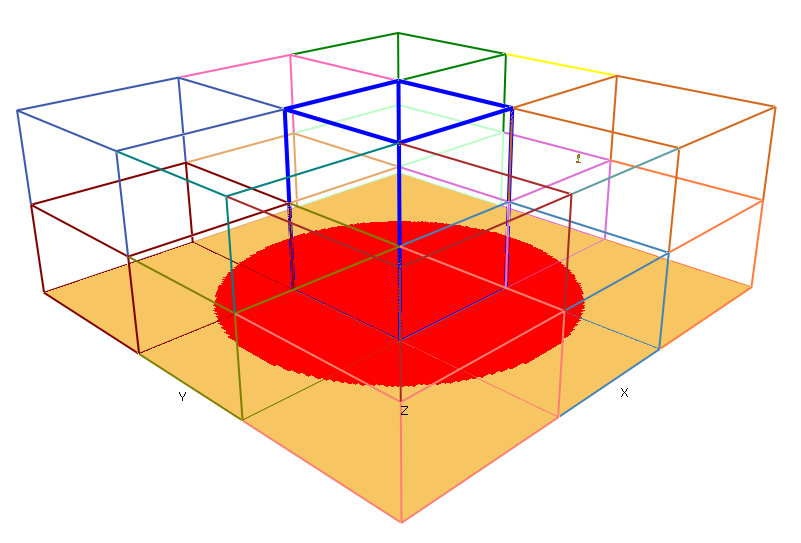
\includegraphics[width=0.83\textwidth]{images/ModellmitgrBrandherd.png}
    \caption{Mesheinteilung bei Modell mit 3 m Raumhöhe und max. spez. Wärmefreisetzungsrate}
    \label{fig:MesheinteilungmitgrBrandherd}
\end{figure}
Die rote Fläche stellt die gesamte Brandfläche bei 300~s dar. Es ist zu erkennen, dass der Brand ab einem gewissen Zeitpunkt die Grenzen des inneren Mesh überschreiten und gegen Ende der Simulationszeit in alle unteren Mesh vorgedrungen sein wird. Laut dem FDS User Guide sollte vermieden werden, dass die Brandfläche verschiedene Mesh berührt \cite[S. 40]{FDSUser}. Dies muss bei der Auswertung der Ergebnisse berücksichtigt werden.

Um den Einfluss dieses Brandherdes mit einer geringeren maximalen spezifischen Wärmefreisetzungsrate zu untersuchen, wird der zeitliche Verlauf der Sprinklerelementtemperatur bei verschiedenen Raumhöhen mit den Daten aus Kap. \ref{sec:VergleichSimulationundBerechnung} in Abb. \ref{fig:AltBrandherdVerlauf} verglichen. 
\begin{figure}
    \centering
    \includegraphics[width=\textwidth]{images/AltBrandherdVerlauf.pdf}
    \caption{Vergleich der Sprinklerelementtemperatur zwischen Simulationen mit $\Dot{q}_{max}=500$~kW/m² (Sim.*) und $\Dot{q}_{max}=5386$~kW/m² (Sim.) bei verschiedenen Raumhöhen.}
    \label{fig:AltBrandherdVerlauf}
\end{figure}
Während die beiden Verläufe mit $H=3$~m bis ca. 170~s so gut wie keine Abweichungen aufweisen, besteht ab diesem Zeitpunkt eine deutliche Divergenz. Die Elementtemperatur der Simulation mit $\Dot{q}_{max}=500$~kW/m² weicht stark vom bis dahin exponentiellen Verlauf ab und folgt bis zum Ende der Simulation einem schwächeren, annähernd linearen Verlauf. 
Allerdings beträgt die Sprinklerelementtemperatur zum Zeitpunkt von 170~s bei beiden Brandherden schon über 125~°C und die Abweichung hat nur noch einen Einfluss auf die Sprinklerköpfe mit einer Nennöffnungstemperatur von 141~°C \bzw 182~°C. 


Bei den Verläufen mit 6~m und 8~m ist keine große Abweichung erkennbar. Dies wird auch ersichtlich in Tab. \ref{tab:altBrandherdErgebnisse}, welche die Ergebnisse der verschiedenen Auslösezeiten zusätzlich noch mit den Berechnungen nach SFPE-Handbook und VDI-Tabelle vergleicht.
\begin{table}\centering
\caption{Vergleich der Sprinklerauslösezeiten (in s) zwischen Simulationen mit $\Dot{q}_{max}=500$~kW/m² (Sim.*), $\Dot{q}_{max}=5386$~kW/m² (Sim.), Berechnungen nach SFPE-Handbuch und VDI-Tabellenwerten für verschiedene Nennöffnungstemperaturen (Trd; in °C)  und Raumhöhen ($\alpha=0{,}047$~kW/s², RTI $=50$~(m/s)$^{0,5}$).}
\label{tab:altBrandherdErgebnisse}
\begin{tabu} to 0.7\textwidth{@{}X[c]X[c]X[c]X[c]X[c]X@{}} \toprule
Trd                 &       & H = 3 m & H = 6 m          & H = 8 m          \\
    \midrule
\multirow{4}{*}{57} & Sim.* & 105     & 142              & 163              \\
                    & Sim.  & 102     & 143              & 170              \\
                    & SFPE  & 104     & 135              & 157              \\
                    & VDI   & 105     & 140              & 160              \\
                    \midrule
\multirow{4}{*}{68} & Sim.* & 115     & 163              & 192              \\
                    & Sim.  & 116     & 165              & 194              \\
                    & SFPE  & 116     & 153              & 179              \\
                    & VDI   & 120     & 155              & 185              \\
                    \midrule
\multirow{4}{*}{79} & Sim.* & 127     & 183              & 221              \\
                    & Sim.  & 126     & 183              & 212              \\
                    & SFPE  & 126     & 169              & 200              \\
                    & VDI   & 130     & 175              & 205              \\
                    \midrule
\multirow{4}{*}{93} & Sim.* & 144     & 209              & 252              \\
                    & Sim.  & 140     & 210              & 259              \\
                    & SFPE  & 139     & 189              & 226              \\
                    & VDI   & 140     & 195              & 230              \\
                    \midrule
\multirow{4}{*}{141}& Sim.* & 188     & 289              & \textgreater 300 \\
                    & Sim.  & 189     & 271              & \textgreater 300 \\
                    & SFPE  & 178     & 252              & 306              \\
                    & VDI   & 180     & 260              & 315              \\
                    \midrule
\multirow{4}{*}{182}& Sim.* & 228     & \textgreater 300 & \textgreater 300 \\
                    & Sim.  & 191     & \textgreater 300 & \textgreater 300 \\
                    & SFPE  & 208     & 301              & 371              \\
                    & VDI   & 215     & 310              & 380              \\
    \bottomrule
\end{tabu}
\end{table}
Differenzen größer 10~s zwischen den beiden Simulationen sind erst ab Nennauslösetemperaturen größer 141~°C zu erkennen. Dabei liegen Auslösezeiten der Simulationen mit $\Dot{q}_{max}=500$~kW/m² aufgrund des flacheren Anstiegs der Sprinklerelementtemperatur grundsätzlich höher.

Abb.~\ref{fig:GastempAltBrandherd} und Abb.~\ref{fig:GasgeschwAltBrandherd} zeigen hierfür den Unterschied in der Gastemperatur und -geschwindigkeit am Sprinklerkopf bei einer Raumhöhe von 3~m auf.
\begin{figure}
    \centering
    \includegraphics[width=0.83\textwidth]{images/AltBrandherdGasTemp.pdf}
    \caption{Verlauf der Rauchgastemperatur am Sprinklerkopf bei verschiedenen max. spez. Wärmefreisetzungsraten mit Sim.: $\Dot{q}_{max}=5386$~kW/m² und Sim.*: $\Dot{q}_{max}=500$~kW/m².}
    \label{fig:GastempAltBrandherd}
\end{figure}
\begin{figure}
    \centering
    \includegraphics[width=0.83\textwidth]{images/AltBrandherdGasGeschw.pdf}
    \caption{Verlauf der Rauchgasgeschwindigkeit am Sprinklerkopf bei verschiedenen max. spez. Wärmefreisetzungsraten mit Sim.: $\Dot{q}_{max}=5386$~kW/m² und Sim.*: $\Dot{q}_{max}=500$~kW/m².}
    \label{fig:GasgeschwAltBrandherd}
\end{figure}
Ab ca. 170~s steigt die Gastemperatur mit $\Dot{q}_{max}=5386$~kW/m² stärker an als die Temperatur mit $\Dot{q}_{max}=500$~kW/m². Grund dafür ist die niedrigere spezifische Wärmefreisetzungsrate der Simulation mit $\Dot{q}_{max}=500$~kW/m². Da mit der im Verhältnis größeren Brandfläche auch ein größerer Plume entsteht, wird mehr Luft induziert und erwärmt. Dies führt zu einer niedrigeren Gastemperatur und somit auch zu einer niedrigeren Sprinklerelementtemperatur. Die Geschwindigkeit des Deckenstrahls erhöht sich dabei, da ein größeres Rauchvolumen an die Decke strömt. 
Ein weiterer Faktor für die Abweichung könnte auf eine Limitierung des Simulationmodells hinweisen. Da bei einer großen Brandfläche die für diese Arbeit definierte Mesheinteilung nicht ideal ist und der Brandherd ab 219~s die Meshgrenzen überschreitet, kann es zu Datenverlusten und Fehlern in der Simulation kommen.

Die Bedeutung der Brandherdgröße und maximalen spezifischen Wärmefreisetzungsrate muss in nachfolgenden Arbeiten näher betrachtet werden. Allerdings kann ausgesagt werden, dass vor allem in der Anfangsphase auch Simulationen mit einer größeren Brandherdgröße zu sehr guten Übereinstimmungen mit den Berechnungen nach SFPE-Handbook führen. 







%%%%%%%%%%%%%%%%%%%%%%%%%%%%%%%%%%%%%%%%%%%%%%%%
\FloatBarrier
\section{Visuelle Auswertung}
\label{VisuelleAuswertung}

Abb.~\ref{fig:visA} zeigt den gesamten Verlauf der Simulation mit Sprinkleraktivierung. Die Wärmefreisetzungsrate von 1~kW wird Abb.~\ref{fig:visA1} überschritten und der Brand beginnt. Der Plume des Feuers steigt auf, erreicht die Decke und der Rauch breitet sich radial an der Decke aus. In Abb.~\ref{fig:visA3} ist zu erkennen, dass der gesamte Deckenbereich mit Rauch gefüllt ist und sich eine Rauchgasschicht und raucharme Schicht etabliert hat. Bei 122,4~s hat das Sprinklerauslöseelement die Nennöffnungstemperatur von 68~°C erreicht und der Sprinklerkopf löst aus. Wasser wird rundum verteilt und verhindert ein weiteres Ausbreiten des Feuers. Die Wärmefreisetzungsrate wird begrenzt.
\begin{figure}[h]\centering
\subfigure[][]{%
\label{fig:visA1}%
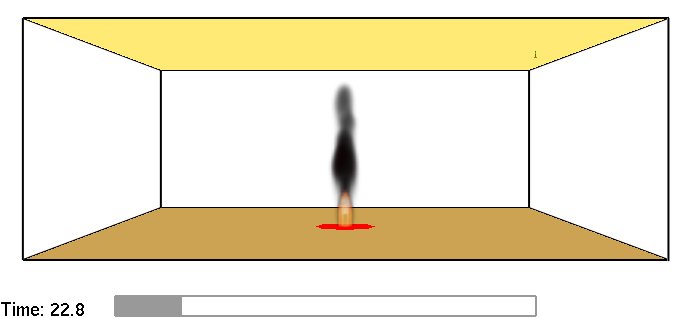
\includegraphics[width=.48\textwidth]{images/FDSBilder/VisuelleAuswertung1.png}}%
\hspace{8pt}%
\subfigure[][]{%
\label{fig:visA2}%
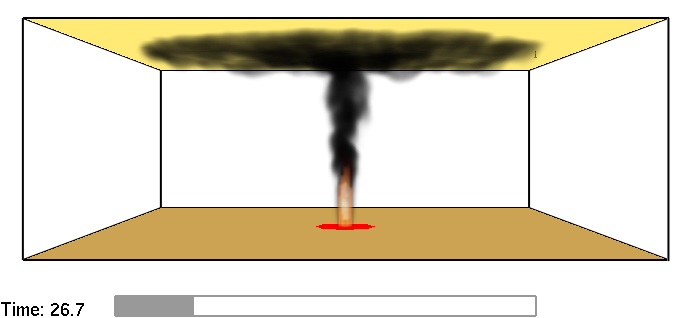
\includegraphics[width=.48\textwidth]{images/FDSBilder/VisuelleAuswertung2.png}}\\
\subfigure[][]{%
\label{fig:visA3}%
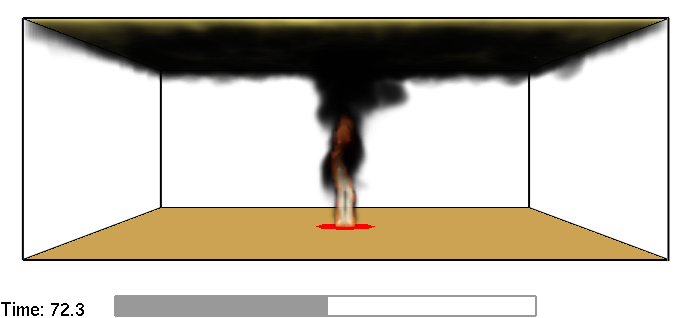
\includegraphics[width=.48\textwidth]{images/FDSBilder/VisuelleAuswertung3.png}}%
\hspace{8pt}%
\subfigure[][]{%
\label{fig:visA4}%
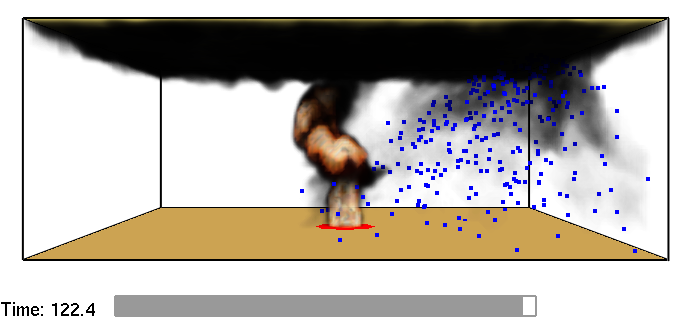
\includegraphics[width=.48\textwidth]{images/FDSBilder/VisuelleAuswertung4.png}}%
\caption{Brandverlauf mit Sprinkleraktivierung in Smokeview (H = 3~m, $\alpha=0,047$ kW/s², C = 0, Trd = 68~°C).}%
\label{fig:visA}%
\end{figure}

FDS ermöglicht es mithilfe der Plot3D Funktion, Vektoren für jede einzelne Zelle in Smokeview simulieren zu lassen. Abb.~\ref{fig:VektorenPlume} stellt den Plume und Ceiling Jet in der Vektoransicht bei 70~s dar. Es ist zu erkennen, dass der aus dem Brand entstandene Rauch mit hoher Geschwindigkeit an die Decke steigt. Kalte Umgebungsluft wird in Plume induziert und kühlt diesen ab. Eine große Verwirbelung auf der linken Seite des Plumes ist auszumachen. Auch am Ceiling Jet selbst wird Luft induziert. Das Rauchgas ist deutlich abgekühlt, wenn es den Sprinklerkopf erreicht. 
\begin{figure}
    \centering
    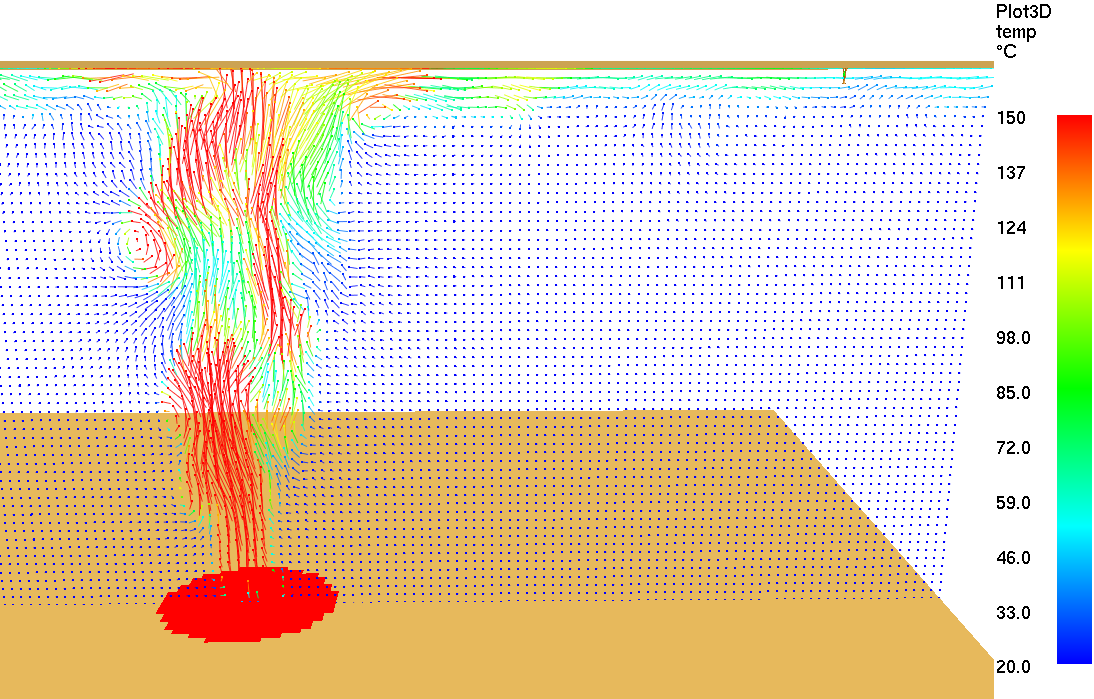
\includegraphics[width=\textwidth]{images/FDSBilder/VektorenPlume.png}
    \caption{Vektordarstellung bei Sekunde 70 (H = 3~m, $\alpha=0,047$ kW/s², C = 0, Trd = 68~°C).}
    \label{fig:VektorenPlume}
\end{figure}
Eine nähere Betrachtung des Bereiches um den Sprinklerkopf herum, zeigt zum selben Zeitpunkt, die Verwirbelungen um den Sprinklerkopf herum auf (siehe Abb.~\ref{fig:VektorenSprinkler}). Wellen heißer Luft erreichen das Auslöseelement. Dieses wird meist horizontal aus Richtung des Brandherdes angeströmt.
\begin{figure}
    \centering
    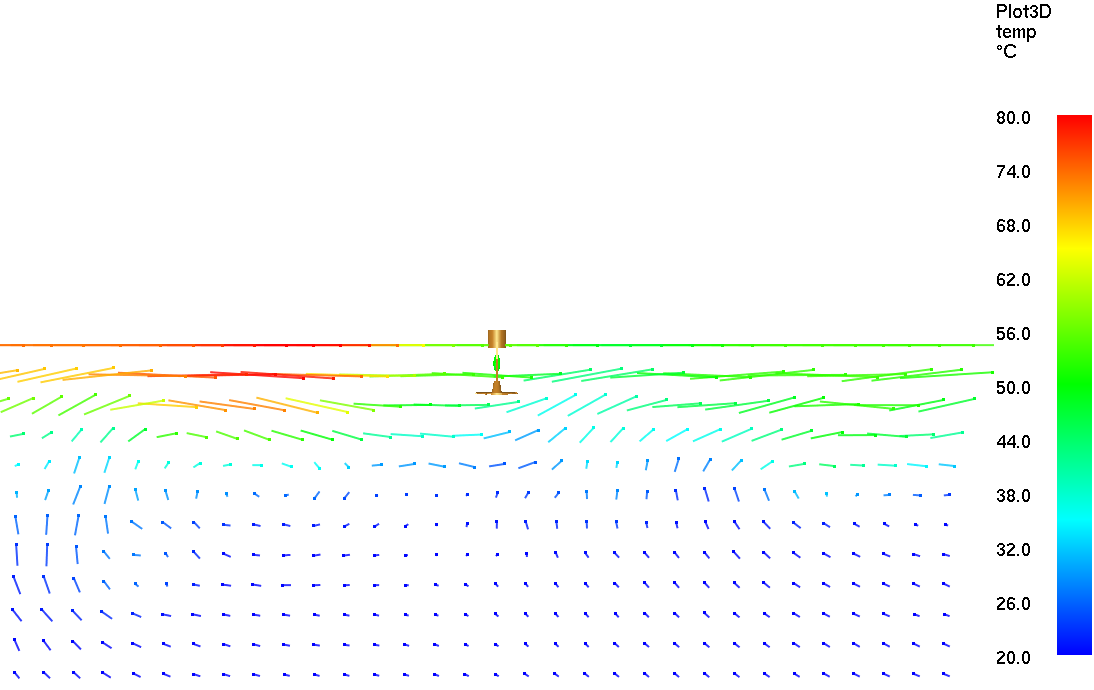
\includegraphics[width=\textwidth]{images/FDSBilder/VektorSprinklerkopf.png}
    \caption{Vektordarstellung am Sprinklerkopf bei Sekunde 70 (H = 3~m, $\alpha=0,047$ kW/s², C = 0, Trd = 68~°C).}
    \label{fig:VektorenSprinkler}
\end{figure}
\clearpage
\SuperPar
Abb.~\ref{fig:PlumeTemp} zeigt eine weitere Anwendung der Plot3D Funktion in Smokeview. Hierbei werden alle Zellenpunkte, die eine bestimmte Temperatur aufweisen, miteinander verbunden und schattiert. In diesem Fall wird die Isofläche des 62,8~°C heißen Rauchgases bei 70~s dargestellt. Man erkennt den aufsteigenden Plume und Ceiling Jet und die relativ gleichmäßige Verteilung an der Decke. Die Verwirbelung an der linken Seite des Plumes aus Abb.~\ref{fig:VektorenPlume} ist ebenfalls zu erkennen.
\begin{figure}[h]
    \centering
    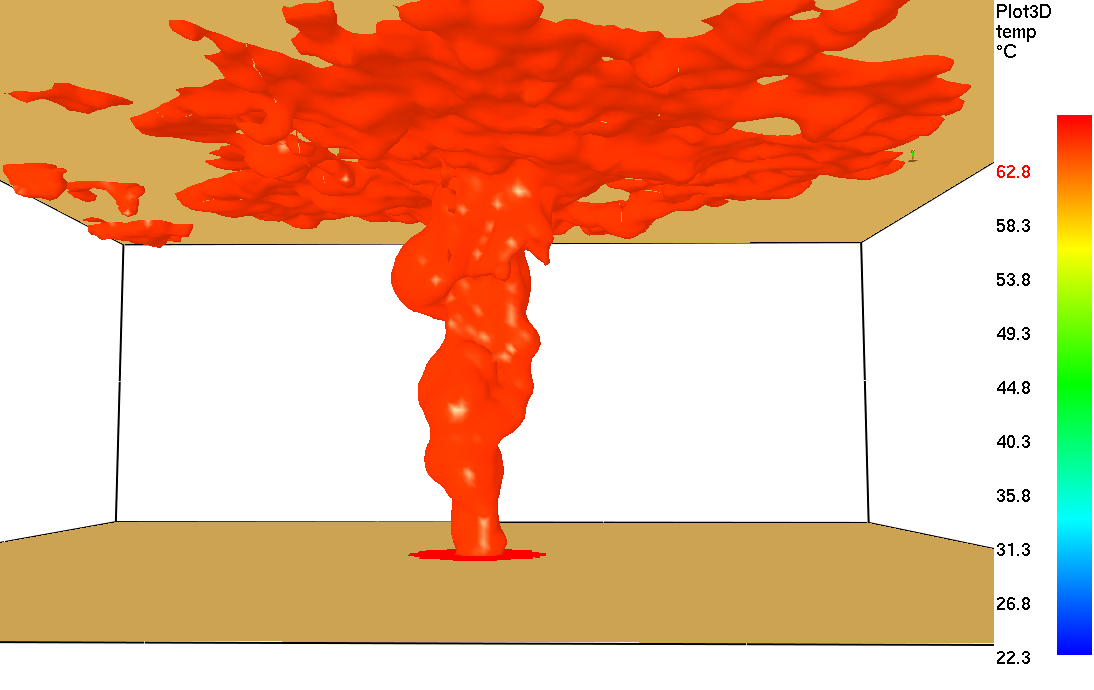
\includegraphics[width=\textwidth]{images/FDSBilder/PlumeTemp.png}
    \caption{Vektordarstellung am Sprinklerkopf bei Sekunde 70 (H = 3~m, $\alpha=0,047$ kW/s², C = 0, Trd = 68~°C).}
    \label{fig:PlumeTemp}
\end{figure}
\clearpage
\SuperPar
Zuletzt wird in Abb.~\ref{fig:PlotEcken} die Isoflächen der Luftgeschwindigkeit untersucht. Die dargestellten Flächen, besitzen eine Luftgeschwindigkeit von 0,04~m/s bei 70~s der Simulation. In der Mitte des Raumes ist die Luftgeschwindigkeit, außer ein paar kleine Ausnahmen, schneller als 0,04~m/s und in den Ecken des Raumes langsamer als dieser Wert. Es scheint, dass die Nachströmung der Luft nicht gleichmäßig aus allen Richtungen erfolgt. Da der Brandherd eine kreisförmige Fläche besitzt, müsste die Luft auch aus den Ecken strömen. Dies ist wahrscheinlich auf die mangelhafte Druckauflösung von FDS an den Raumgrenzen zurückzuführen.

\begin{figure}[h]
    \centering
    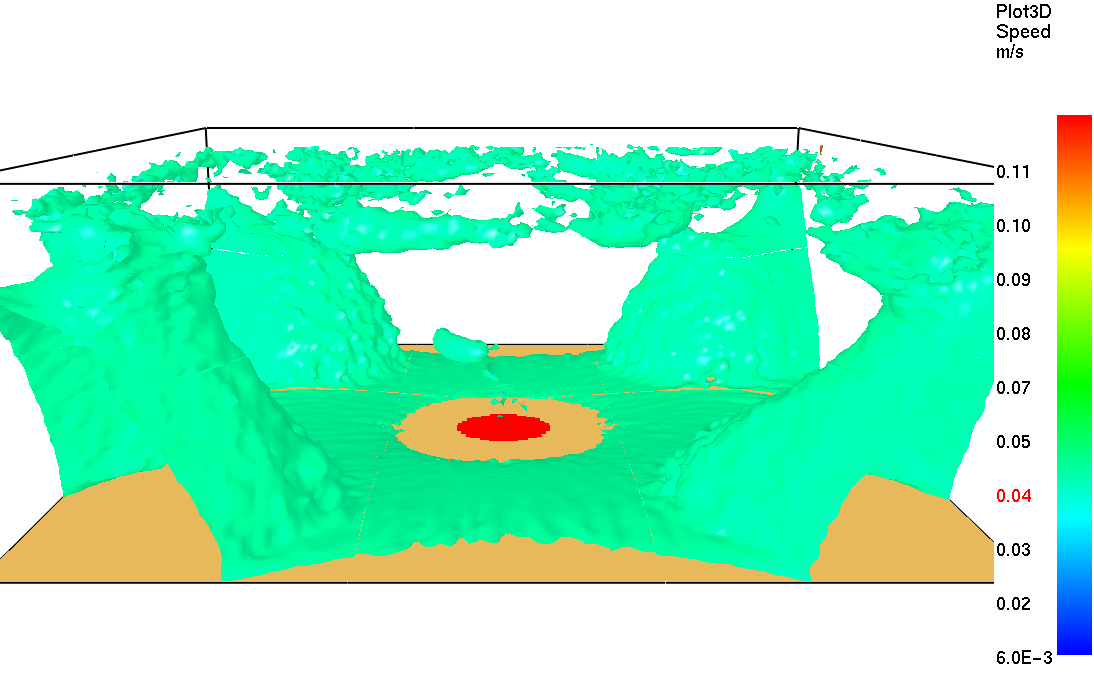
\includegraphics[width=\textwidth]{images/FDSBilder/PlotEcken.png}
    \caption{Vektordarstellung am Sprinklerkopf bei Sekunde 70 (H = 3~m, $\alpha=0,047$ kW/s², C = 0, Trd = 68~°C).}
    \label{fig:PlotEcken}
\end{figure}













\begin{comment}
\begin{figure}%
\centering
\subfigure[][]{%
\label{fig:visA1}%
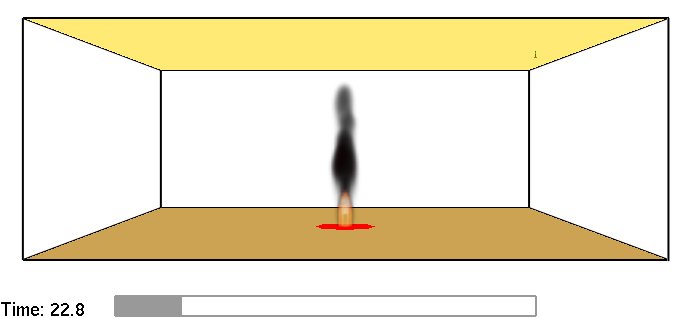
\includegraphics[width=.45\textwidth]{images/FDSBilder/VisuelleAuswertung1.png}}%
\hspace{8pt}%
\subfigure[][]{%
\label{fig:visA2}%
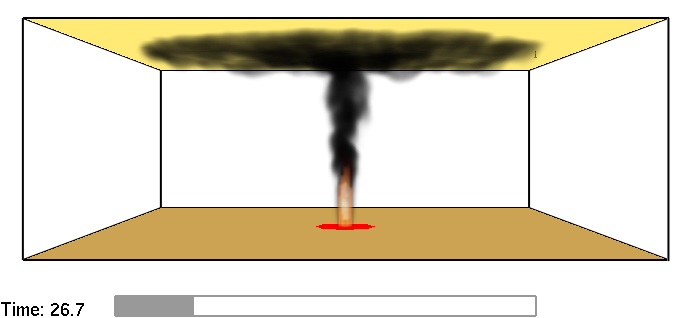
\includegraphics[width=.45\textwidth]{images/FDSBilder/VisuelleAuswertung2.png}}\\
\subfigure[][]{%
\label{fig:visA3}%
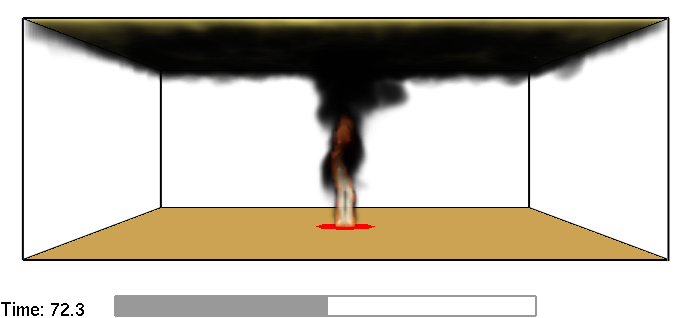
\includegraphics[width=.45\textwidth]{images/FDSBilder/VisuelleAuswertung3.png}}%
\hspace{8pt}%
\subfigure[][]{%
\label{fig:visA4}%
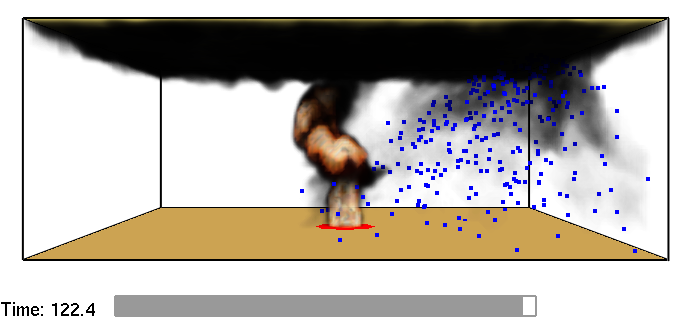
\includegraphics[width=.45\textwidth]{images/FDSBilder/VisuelleAuswertung4.png}}%
\caption{Brandverlauf mit Sprinkleraktivierung bei H = 3~m, $\alpha=0,047$ kW/s², C = 0, Trd = 68~°C.
\subref{fig:visA1} describes the first subfigure;
\subref{fig:visA2} describes the second subfigure;
\subref{fig:visA3} describes the third subfigure;
and,\subref{fig:visA4} describes the last subfigure.}%
\label{fig:visA}%
\end{figure}
\end{comment} 

